\documentclass[tikz,border=20pt]{standalone}
\usepackage{amsmath,amssymb}
\usepackage{tikz}
\usetikzlibrary{arrows.meta,calc}

\begin{document}
	
	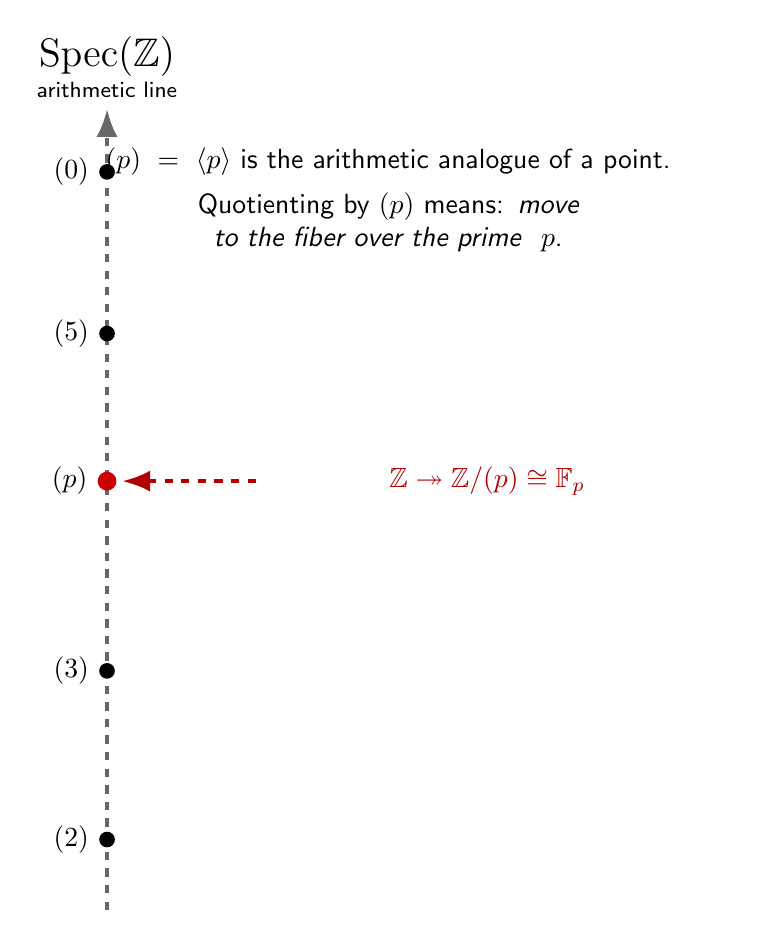
\begin{tikzpicture}[
		x={(1cm,0cm)},
		y={(0.65cm,0.38cm)},
		z={(0cm,1.7cm)},
		scale=1.05,
		font=\sffamily,
		>=Latex,
		pt/.style={circle, fill=black, inner sep=2pt},
		sel/.style={circle, fill=red!80!black, inner sep=2.4pt}
		]
		
		% Vertical arithmetic axis
		\draw[->, ultra thick, dashed, gray!80!black]
		(0,0,-0.5) -- (0,0,5.2)
		node[above, align=center, text=black]
		{\Large $\operatorname{Spec}(\mathbb{Z})$\\[-1pt]\footnotesize arithmetic line};
		
		\node[pt, label=left:{$(2)$}] at (0,0,0.0) {};
		\node[pt, label=left:{$(3)$}] at (0,0,1.2) {};
		\node[sel, label=left:{$(p)$}] at (0,0,2.55) {};
		\node[pt, label=left:{$(5)$}] at (0,0,3.6) {};
		\node[pt, label=left:{$(0)$}] at (0,0,4.75) {};
		
		% quotient label
		\draw[->, ultra thick, dashed, red!70!black] (1.8,0,2.55) -- (0.18,0,2.55);
		\node[align=left, text=red!70!black] at (4.6,0,2.55)
		{$\mathbb Z\twoheadrightarrow \mathbb Z/(p)\cong \mathbb F_p$};
		
		% caption
		\node[align=center, text width=8.8cm] at (3.4,0,4.55)
		{$\displaystyle (p)=\langle p\rangle$ is the arithmetic analogue of a point.\\[4pt]
			Quotienting by $(p)$ means: \emph{move to the fiber over the prime } $p$.};
		
	\end{tikzpicture}
	
\end{document}